\documentclass[conference]{IEEEtran}
\usepackage[utf8]{inputenc}
\usepackage{amsmath,amsfonts,amssymb}
\usepackage{graphicx}
\usepackage{hyperref}
\usepackage{booktabs}
\usepackage{array}
\usepackage{tabularx}

\title{Survey on Semantic and Multimodal Information Retrieval}

\author{}

\begin{document}

\maketitle



\begin{abstract}
The massive spreading of digital content across diverse forms of media has heightened the stakes on retrieval processes that can comprehend and traverse information in semantically relevant and modality-sensitive language. Keyword-based search engines are handicapped when handling multimodal documents or when attempting to decipher user intent from a multiplicity of data types. The current review encompasses the theoretical and background context of semantic and multimodal information retrieval and provides a stage for more extensive study. We start our analysis by exploring two classic research papers that have greatly influenced early perspectives in this discipline. These papers form the basis of the large body of subsequent literature, including the wide variety of modern methodologies and advances in the field. As research in artificial intelligence and machine learning has evolved, so too have the tools for semantic understanding and multimodal fusion. Recent approaches leverage deep learning to align textual, visual, and auditory modalities, offering powerful new capabilities for precise and intuitive information retrieval across domains.
\end{abstract}

\begin{IEEEkeywords}
Semantic Retrieval, Multimodal Information Retrieval, Deep Learning, Cross-modal Search, Survey
\end{IEEEkeywords}

\section{Introduction}
The field of information retrieval (IR) has traveled a great distance since the arrival of enormous amounts of heterogeneous multimedia content. Users nowadays no longer deal just with text-based information; rather, they need to be able to search and get meaningful interpretation from images, videos, audio files, and other non-text data. Modern-day retrieval systems, therefore, need to possess the ability to interpret and bring together different sources of data without losing semantic significance.

This introduces the need for systems that incorporate multimodal processing and semantic comprehension. The ability to bridge text to image content, or connect natural language queries with video data, demands sophisticated architecture beyond lexical matching. The aim of this survey is to provide a conceptual and historical basis for such systems; this introduction section thus provides the background and motivation for a much larger investigation of the state-of-the-art in semantic multimodal retrieval, which is discussed in greater detail in the Related Works section.

\subsection*{Basic Concepts}

\textbf{Modality:} Refers to the form in which data is represented, such as text, image, video, or audio.

\textbf{Multimodal Data:} Data that includes two or more modalities. For instance, a webpage with both images and captions, or a video containing speech, visuals, and subtitles.

\textbf{Semantic Retrieval:} Retrieval based on the meaning and context of content, not merely syntactic forms or keywords. Semantic retrieval aims to understand the user's intent and the content's conceptual framework.

\section{Background and Foundational Works}

\subsection{Intelligent Indexing and Semantic Retrieval of Multimodal Documents}
This seminal work discusses early efforts at introducing semantic interpretation into multimodal indexing. The authors propose a conceptual framework wherein multimodal documents are indexed both to their native data types and to inferences made regarding their semantic meaning \cite{pfeffer2001intelligent}. Their system integrates text, image, and layout cues to form a semantically richer representation of documents.

\subsubsection{Indexing Architecture}
The paper introduces a layered indexing architecture where each modality is first processed separately to extract modality-specific features. For example, textual data undergoes natural language processing to extract key concepts, while images are analyzed for visual patterns and object recognition. These features are then fused into a unified semantic index.

\subsubsection{Semantic Alignment}
One of the key contributions of this paper is that it tries to get various modalities into alignment at the conceptual level. Instead of dealing with modalities as independent attributes, the system presented here tries to find shared semantic concepts. For instance, a picture of a "mountain" and the caption "snowy peak" are semantically identical despite their difference in modality.

\subsubsection{Query Processing and Retrieval}
User queries are searched in a comparable semantic manner. A query may be a collection of text keywords, a sample image, or both. Retrieval entails mapping these queries onto a semantically indexed space so that cross-modal retrieval can be enabled. For example, a text query may produce corresponding images, or an image input may result in documents that are semantically related.

\begin{figure}
    \centering
    
\includegraphics[width=0.7\linewidth]{images/image4.png}
    \caption{Reproduced from Srihari, R. K., Zhang, Z., and Rao, A. (2000). “Intelligent Indexing and Semantic Retrieval of Multimodal Documents.”}
    \label{fig:enter-label}
\end{figure}

\subsubsection{Challenges Identified}
The paper outlines several challenges, including:
\begin{enumerate}
    \item Representing semantics uniformly across modalities.
    \item Scalability of multimodal indexing systems.
    \item Ambiguity in semantic interpretation.
    \item Lack of annotated training data for supervised learning.
\end{enumerate}

Despite being dated, this work sets a precedent for modern systems that aim to learn joint embeddings across modalities using deep learning frameworks.

\subsection{Semantic Search on Text and Knowledge Bases by Hannah Bast et al.}
The main contribution of Bast et al.\cite{bast2016semantic} explores semantic search processes in unstructured textural content and structured knowledge bases (KBs). While the paper's focus is primarily on text information, the architectural and methodological decisions discussed are of general applicability and form the basis for systems that can perform semantic searching across various modalities.

\subsubsection{Entity-Oriented Search and Semantic Representation}
The authors argue that users search for \textit{entities} (people, places, and events, for example) and their interrelations, rather than for disconnected keywords. This view redirects attention from syntactic matching to semantic comprehension. In practice, this means recognizing named entities in searches and anchoring them to structured representations in a knowledge repository—a process called \textit{entity linking}.

Entity disambiguation is important. For instance, the separation of "Apple," the corporation, from "apple," the fruit, needs reasoning dependent on context, which is facilitated by co-occurrence statistics, knowledge graph embeddings, and linguistic patterns.


\subsubsection{Semantic Parsing and Logical Query Mapping}
One of the core contributions of this work is in mapping natural language queries to structured logical forms such as SPARQL. This enables querying complex KBs in a way that preserves the query's intent. The process of semantic parsing involves understanding the grammatical and semantic structure of a sentence and aligning it to formal relations in the KB schema.

This aligns well with the broader goals of semantic search engines that must handle ambiguous or vague queries, especially in multimodal settings. A visual or audio query, just like a textual one, can benefit from an intermediate logical representation or latent semantic space.

\subsubsection{Hybrid Search: Combining KBs with Full-Text}
Bast et al. note that even rich KBs are not complete. To help improve recall, the system returns both KB query results and full-text search results over a collection of unstructured documents. This hybrid retrieval approach acknowledges the fact that not all semantic relations are present in structured form. For instance, a new fact about a celebrity might be found in news text prior to its addition to a KB.

This is particularly interesting in multimodal search. Also, when image tags or transcripts of audio do not have semantic tags, fallback methods may employ full-text document retrieval or caption search to improve result quality.

\subsubsection{System Architecture and Design Principles}
The system architecture described includes:
\begin{enumerate}
    \item High-performance indexing of RDF triples from KBs.
    \item Named entity recognition and linking tools.
    \item A query parser that converts natural language into logical queries.
    \item A scoring function that ranks answers from both KB and full-text sources.
\end{enumerate}

This architecture embodies a modular and extensible semantic search approach, an important requirement for systems working over heterogeneous modalities. For instance, a multimodal system can swap the full-text index for a multimodal embedding space or use vision-language models in place of text-based entity linkers.


\subsubsection{Extending to Multimodal Scenarios}
Although the paper's scope is limited to text and knowledge bases, its insights are foundational for multimodal systems. Consider the following parallels:
\begin{enumerate}
    \item \textbf{Entity Linking Across Modalities:} An image may contain a face that corresponds to an entity in a KB; similarly, a video transcript might mention locations or events that need disambiguation.
    \item \textbf{Semantic Parsing from Non-Textual Inputs:} Just as natural language is parsed into structured queries, visual scenes or audio patterns can also be parsed into semantic representations using modern deep learning techniques.
    \item \textbf{Hybrid Modal Search:} When structured annotations or object tags are insufficient, systems can use captions, ASR transcripts, or OCR-extracted text to supplement search.
\end{enumerate}

Thus, the paper provides a theoretical and architectural underpinning for systems that aim to blend semantic reasoning with heterogeneous data inputs. It guides the formulation of scalable, hybrid architectures that can bridge gaps in modality coverage or annotation completeness.



\section{Related Works}

This section discusses 18 major research papers that have significantly contributed to semantic and multimodal information retrieval. They are presented in chronological order, and each is elaborated in detail to provide a clear and comprehensive understanding.

\begin{enumerate}

\item \textbf{DeViSE (2013)} – Frome et al. \cite{frome2013devise} introduced the Deep Visual-Semantic Embedding Model (DeViSE), which represented a breakthrough in connecting visual and linguistic domains. Traditional image classification models were limited to predefined categories, but DeViSE pioneered a new approach by projecting images and words into a shared semantic embedding space.
The architecture consists of two main components: a convolutional neural network (CNN) trained on ImageNet to extract visual features, and a skip-gram model (Word2Vec) that provides distributed word representations. The innovation lies in how these components are connected. Rather than training the CNN to predict discrete class labels, DeViSE trains it to map images to the same semantic space as word vectors. This mapping is learned using a ranking loss function that ensures images are positioned close to their corresponding labels in the embedding space.
What makes DeViSE particularly powerful is its ability to perform zero-shot recognition. Since images and words share the same semantic space, the model can recognize objects it has never seen before during training, as long as there exists a textual description or word embedding for that object. For example, if the model was trained on "cat" but not "tiger," it could still recognize tigers because the word "tiger" exists in the semantic space and shares similarities with "cat."
This capability fundamentally changed how researchers approached multimodal retrieval. With DeViSE, users could search for images using text descriptions, even when those exact descriptions were never part of the training data. The model also enabled semantic image search, where results are ranked based on conceptual similarity rather than just visual appearance.
DeViSE demonstrated that meaningful cross-modal connections could be established through learned embeddings, paving the way for more sophisticated approaches to semantic and multimodal retrieval. Its impact extends beyond academic research into practical applications like content-based image retrieval systems and accessible image search engines that support natural language queries.


\item \textbf{Unifying Visual-Semantic Embeddings with Multimodal Neural Language Models (2014)} – Kiros et al. \cite{kiros2014unifying} proposed a novel approach that unites computer vision and natural language processing through the confluence of neural language models and visual-semantic embeddings. The research was one of the key contributions in multimodal learning in that it came up with an umbrella under which images and text could be expressed within a common semantic space.

The authors tackled a basic problem in multimodal learning: although earlier visual-semantic embedding models were able to link images with relevant text, they were unable to create new descriptions or reason about visual content. On the other hand, language models were able to produce coherent text but without visual grounding. This work sought to bring these strands together to develop systems capable of both comprehending and generating language about visual content.
The framework consists of three main components:
\begin{enumerate}
\item \textbf{Visual encoder:} A convolutional neural network (CNN) that extracts image features, specifically using a pre-trained model on ImageNet.
\item \textbf{Embedding space:} A joint embedding layer that maps both visual features and textual features into a common semantic space.
\item \textbf{Neural language model:} A recurrent neural network (RNN) that can generate text conditioned on visual content.
\end{enumerate}
The key innovation was the integration of these components into a coherent framework. The model was trained on image-caption pairs, learning to:
\begin{enumerate}
\item Map images and their descriptions to nearby points in the joint embedding space.
\item Generate appropriate captions for images by conditioning the language model on visual features.
\item Maintain semantic coherence between visual and textual modalities.
\end{enumerate}
This approach enabled several capabilities that were novel for 2014:
\begin{enumerate}
\item \textbf{Bidirectional retrieval:} The ability to retrieve relevant images given text queries and vice versa.
\item \textbf{Image caption generation:} Producing natural language descriptions of image content.
\item \textbf{Multimodal similarity:} Computing semantic similarity between images and text based on their meaning rather than just surface features.
\item \textbf{Structure-preserving mapping:} Maintaining semantic relationships in the embedding space (e.g., images of "running dogs" would be closer to text about "dogs running" than to unrelated concepts).
\end{enumerate}
The authors demonstrated their system on tasks including image-text retrieval and caption generation using datasets like Flickr8K, Flickr30K, and COCO. The results showed that unifying visual semantics with language models improved performance on both retrieval and generation tasks compared to models that handled these tasks independently.
Some key technical aspects of the work included:
\begin{enumerate}
\item \textbf{Contrastive learning:} Using a ranking loss function to ensure that matched image-text pairs had higher similarity scores than unmatched pairs.
\item \textbf{Log-bilinear language model:} A specific type of neural language model that was effective for modeling word sequences conditioned on visual context.
\item \textbf{Embedding normalization:} Techniques to ensure stable training and meaningful distance metrics in the joint embedding space.
\end{enumerate}
This work was important in the sense that it represented one of the initial efforts to bring visual and textual comprehension together within a comprehensive paradigm, which set the stage for later developments in multimodal learning. The findings indicated how neural models could initiate the creation of a general comprehension of content between modalities, although the capabilities were very limited relative to later systems. The paper inspired a fruitful line of research on multimodal neural networks, and follow-up work created more complex models for cross-modal comprehension and generation.

\begin{figure}
    \centering
    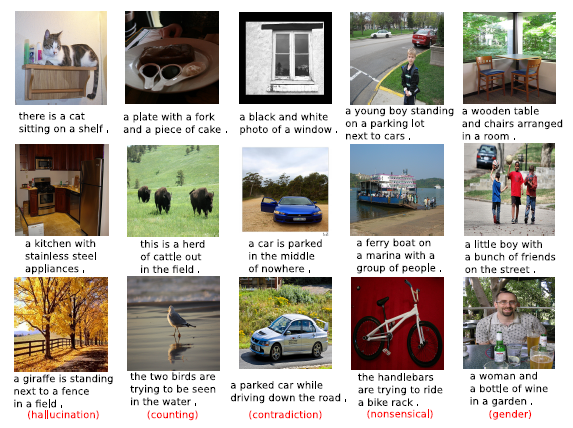
\includegraphics[width=0.9\linewidth]{images/image5.png}
    \caption{Reproduced from Kiros, R., Salakhutdinov, R., and Zemel, R. S. (2014). “Unifying Visual-Semantic Embeddings with Multimodal Neural Language Models.”}
    \label{fig:enter-label}
\end{figure}

\item \textbf{Polysemous Visual-Semantic Embedding for Cross-Modal Retrieval
 (2019)} – Song et al. \cite{song2019polysemous} addressed a critical issue in semantic retrieval, namely polysemy, which pertains to the phenomenon wherein words may possess various distinct meanings contingent upon their context. Conventional embedding models characterize each word through a single vector, which fails to capture semantic distinctions. For instance, the term "bank" may denote either a financial institution or a location adjacent to a river—two distinctly different concepts that ought not to share an identical representation within a semantic framework.
The Polysemous Visual-Semantic Embedding model overcomes this limitation in that words may have multiple embeddings based on their different senses or meanings. In this way, it acknowledges the fact that most of the meaning of a word becomes apparent once used with a visual context. A photo of flowing water adjacent to a green grass field, for example, would make "bank" intelligible in use of its meaning as "riverside."
The model architecture adds a sense disambiguation module that exists in parallel with standard visual and textual encoders. In training, the model is learned to generate multiple sense-specific embeddings for polysemous words. While processing a query or an image, it dynamically selects the most appropriate sense embedding based on context present (visual or textual).
To achieve this, the researchers employed a two-step strategy: first, they clustered image features of polysemous terms to discover different senses; second, they learned separate embeddings for each discovered sense. During retrieval time, the model performs "soft" sense assignment, whereby it considers multiple potential meanings but weighs them according to contextual significance.
This approach greatly improved the accuracy of information retrieval, especially for queries that contain ambiguous terms. In practical use, a person looking up "apple" would receive results neatly sorted into fruit and technology categories, rather than a mixed jumble of both. Additionally, the model improved cross-modal retrieval tasks, where users query with an image and then receive text results (or vice versa).
The Polysemous Visual-Semantic Embedding model highlighted the importance of contextual understanding in multimodal models. Its merits have influenced later work on context-aware embeddings and demonstrated that semantic richness, beyond simple one-to-one matching, is key to effective multimodal retrieval.

\item \textbf{BERT (2019)} – Devlin et al. \cite{devlin2019bert} It has been proposed as a novel language representation model that drastically changes the prevailing paradigm in natural language processing. The model is aimed at resolving a basic limitation of previous language models by making use of bidirectional context so that there could be deeper understanding of language. The main contribution of BERT is
\begin{enumerate}
\item \textbf{Bidirectional training:} As opposed to previous models, where text was processed unidirectionally, either left to right or vice versa, BERT is designed particularly to process both sides of text at once. The bidirectional approach enables this model to develop a deeper understanding of context and word meanings.
\item \textbf{Pre-training and fine-tuning paradigm:} BERT takes recourse to both dual mechanisms, where the model is pretrained on large amounts of unlabeled text by means of two novel unsupervised language tasks (masked language model and next sentence prediction) and then fine-tuned to specific downstream tasks by means of a small set of task-specific parameters.

\item \textbf{Masked language modeling (MLM):} During pre-training, 15% of tokens in each sequence are randomly masked, and the model must predict these masked tokens based on surrounding context. This forces the model to learn rich, bidirectional representations.

\item \textbf{Next sentence prediction (NSP):} BERT is trained to predict whether two sentences appear consecutively in the original text, helping it understand relationships between sentences.

\item \textbf{Transformer-based architecture:} Building on Vaswani et al.'s Transformer model, BERT uses attention mechanisms to weigh the importance of words in relation to each other, regardless of their position in the sentence.
\end{enumerate}
The researchers developed two variants of the model:
\begin{enumerate}
\item \textbf{BERT-Base:} 12 layers, 768 hidden dimensions, 12 attention heads, and 110M parameters.
\item \textbf{BERT-Large:} 24 layers, 1024 hidden dimensions, 16 attention heads, and 340M parameters.
\end{enumerate}
BERT achieved state-of-the-art results on a wide range of NLP tasks, including:
\begin{enumerate}
\item \textbf{Question answering:} Setting new records on the Stanford Question Answering Dataset (SQuAD).
\item \textbf{Natural language inference:} Surpassing previous approaches on the GLUE benchmark.
\item \textbf{Named entity recognition:} Improving performance on CoNLL-2003.
\item \textbf{Sentiment analysis:} Achieving superior results on the SST-2 dataset.
\item \textbf{Text classification:} Demonstrating exceptional performance across various classification tasks.
\end{enumerate}
The impact of BERT on the field of NLP has been profound:
\begin{enumerate}
\item \textbf{New paradigm:} BERT solidified the pre-train/fine-tune paradigm that has become standard in NLP.
\item \textbf{Contextual embeddings:} It demonstrated the power of contextual word representations over static embeddings.
\item \textbf{Architecture foundation:} BERT inspired numerous subsequent models including RoBERTa, ALBERT, DistilBERT, and many others that refined and built upon its core architecture.
\item \textbf{Practical applications:} The model has been deployed in real-world systems including Google Search, improving the engine's understanding of search queries.
\end{enumerate}
The success of BERT can be traced to its ability to learn rich, contextualized language representations using large-scale unsupervised pre-training followed by fine-tuning to specific tasks. This framework allows the model to leverage knowledge between many different natural language processing tasks and requires few adaptation changes to task-specific architecture designs. The model's method of learning bidirectional context has proved to be a game-changer that has influenced virtually every subsequent study in language modeling.

\item \textbf{Sentence-BERT (2019)} – Reimers and Gurevych's efforts at creating Sentence-BERT \cite{reimers2019sentence} represented a significant advance in semantic text representation with important implications for multimodal retrieval systems. While BERT had revolutionized the natural language processing domain with its contextual word embeddings, it was not pre-trained to generate fixed-length sentence representations critical for the purpose of effective similarity determination and retrieval tasks.
Sentence-BERT updates BERT's structure by using siamese and triplet network designs to produce sentence embeddings that capture semantic meaning. It is learned using natural language inference datasets, making it possible for the model to detect contradiction, entailment, and neutral relation between sentences. This particular objective forces the model to learn semantic understanding instead of just encoding syntactic structure.
The key innovation is Sentence-BERT's capacity to produce fixed-dimensional embeddings, typically 768-dimensional, for whole sentences or paragraphs. These can be compared using simple cosine similarity, making the approach computationally feasible for large-scale retrieval tasks. Compared to using the standard BERT for pairwise comparisons, Sentence-BERT reduces the computation time from several days to a few minutes when used on common corpus sizes without sacrificing an equivalent degree of accuracy.
In the context of multimodal information retrieval, Sentence-BERT is an essential element of text encoding. Its combination with visual encoders enables sophisticated text-to-image retrieval by matching text queries in an identical embedding space that comprises images. The ability of the model to capture subtle semantic relationships between sentences is useful in cross-modal applications.
An example would be that a Sentence-BERT encoding of "person playing guitar on stage" would be close to both "concert guitarist" and "musician performing live" in embedding space, regardless of wording variation. This semantic understanding integrated with appropriate visual encoders enables retrieval to link images related to the conceptual content of queries instead of mandating exact keyword matches.
Additionally, Sentence-BERT enables rapid retrieval within large-scale multimodal databases. Its embeddings can be computed and indexed in advance, allowing for speedy similarity searches when a query is received. As a result, this has made it extremely useful for a variety of industrial applications such as content discovery, recommendation, and semantic search engines. The impact of Sentence-BERT extends beyond the scope of academic research since it is an essential foundation of several production systems requiring understanding of text semantics. These comprise multimodal search engines, where text queries should return relevant images, videos, or audio content.

\item \textbf{VisualBERT (2019)} - In their original research, Li et al. \cite{li2019visualbert} introduced VisualBERT, which uses the transformer structure to handle joint analysis of visual and textual information. Unlike previous approaches that preserved individual processing of visual and textural information until later fusion stages, VisualBERT allows for an early integration of these two modalities, thus supporting meaningful cross-modal interaction in the neural network from the start.
The architecture frames image parts as similar to words in a sentence. Specifically, it uses recognized objects or image parts (derived by a pre-trained object detector like Faster R-CNN) and represents these as "visual tokens" alongside text tokens as an integrated sequence. Finally, both modalities pass jointly in parallel by way of several transformer processing layers, allowing for words and image parts to form relations by way of the self-attention mechanism.
Integration comes about by means of several basic elements:


\begin{enumerate}
\item \textbf{Visual embeddings:} Image components are integrated into a framework of dimensions that is compatible with word embeddings.
\item \textbf{Position embeddings:} Both textual and visual modules receive information about position.
\item \textbf{Segment embeddings:} Segments need to be classified as either belonging to the textual or visual modality.
\item \textbf{Self-attention layers:} Enable interaction between each unique module and every other module, regardless of modality.
\end{enumerate}


The transformer-based architecture of VisualBERT enables the model to realize complex relationships between visual and linguistic elements. An example would be understanding, when examining the sentence "The man is riding a bicycle" and an image, that the word "bicycle" can be related to the region of the image representing the bicycle and that "man" can be related to the man in the image.
The model is pre-trained on image-caption pairs with two main goals: masked language modeling, which predicts hidden words conditioned on both text and image context, and image-text matching, which measures how well a caption and an image match. This pre-training stage strengthens the model's ability to understand vision-language relations before it is fine-tuned for specific tasks. In semantic retrieval, VisualBERT has proved that transformer models can successfully represent both visual and text-based information within one semantic framework. This representation scales precision in cross-modal retrieval, where semantic content, and not superficial features, drives relevancy. The impact of VisualBERT existed beyond its immediate results; it led to the development of the "vision-language transformer" paradigm, now dominating studies in multimodal artificial intelligence. Its formulation showed the power of using the self-attention mechanism to derive strong intermodal connections, consequently influencing a wide range of subsequent models built to perform activities like multimodal search, visual question answering, and image captioning. This practice showed that processing multiple modalities concurrently in an initial phase was superior to late fusion.


\item \textbf{DeepStyle (2019)} – Tautkute et al. \cite{tautkute2019deepstyle} DeepStyle is a domain-specific multimodal search engine for the fashion world and an example of semantic understanding realized in areas where subjective and aesthetic attributes prevail. In contrast to many multimodal retrieval systems that focus on tangible object categories or empirical connections, DeepStyle deals with the complexity of retrieving items based on intangible concepts like style, aesthetic appeal, and fashion sense.
The system uses convolutional neural networks to extract visual features and text encoders to analyze descriptive text content to enable mapping of both modalities to a common embedding space. DeepStyle differs in its training process where it uses human judgements of stylistic similarity to structure the embedding space. To aid in this study, the researchers created a large dataset of fashion items, style-related features, and ratings of stylistic similarity by users.

\begin{figure}
    \centering
    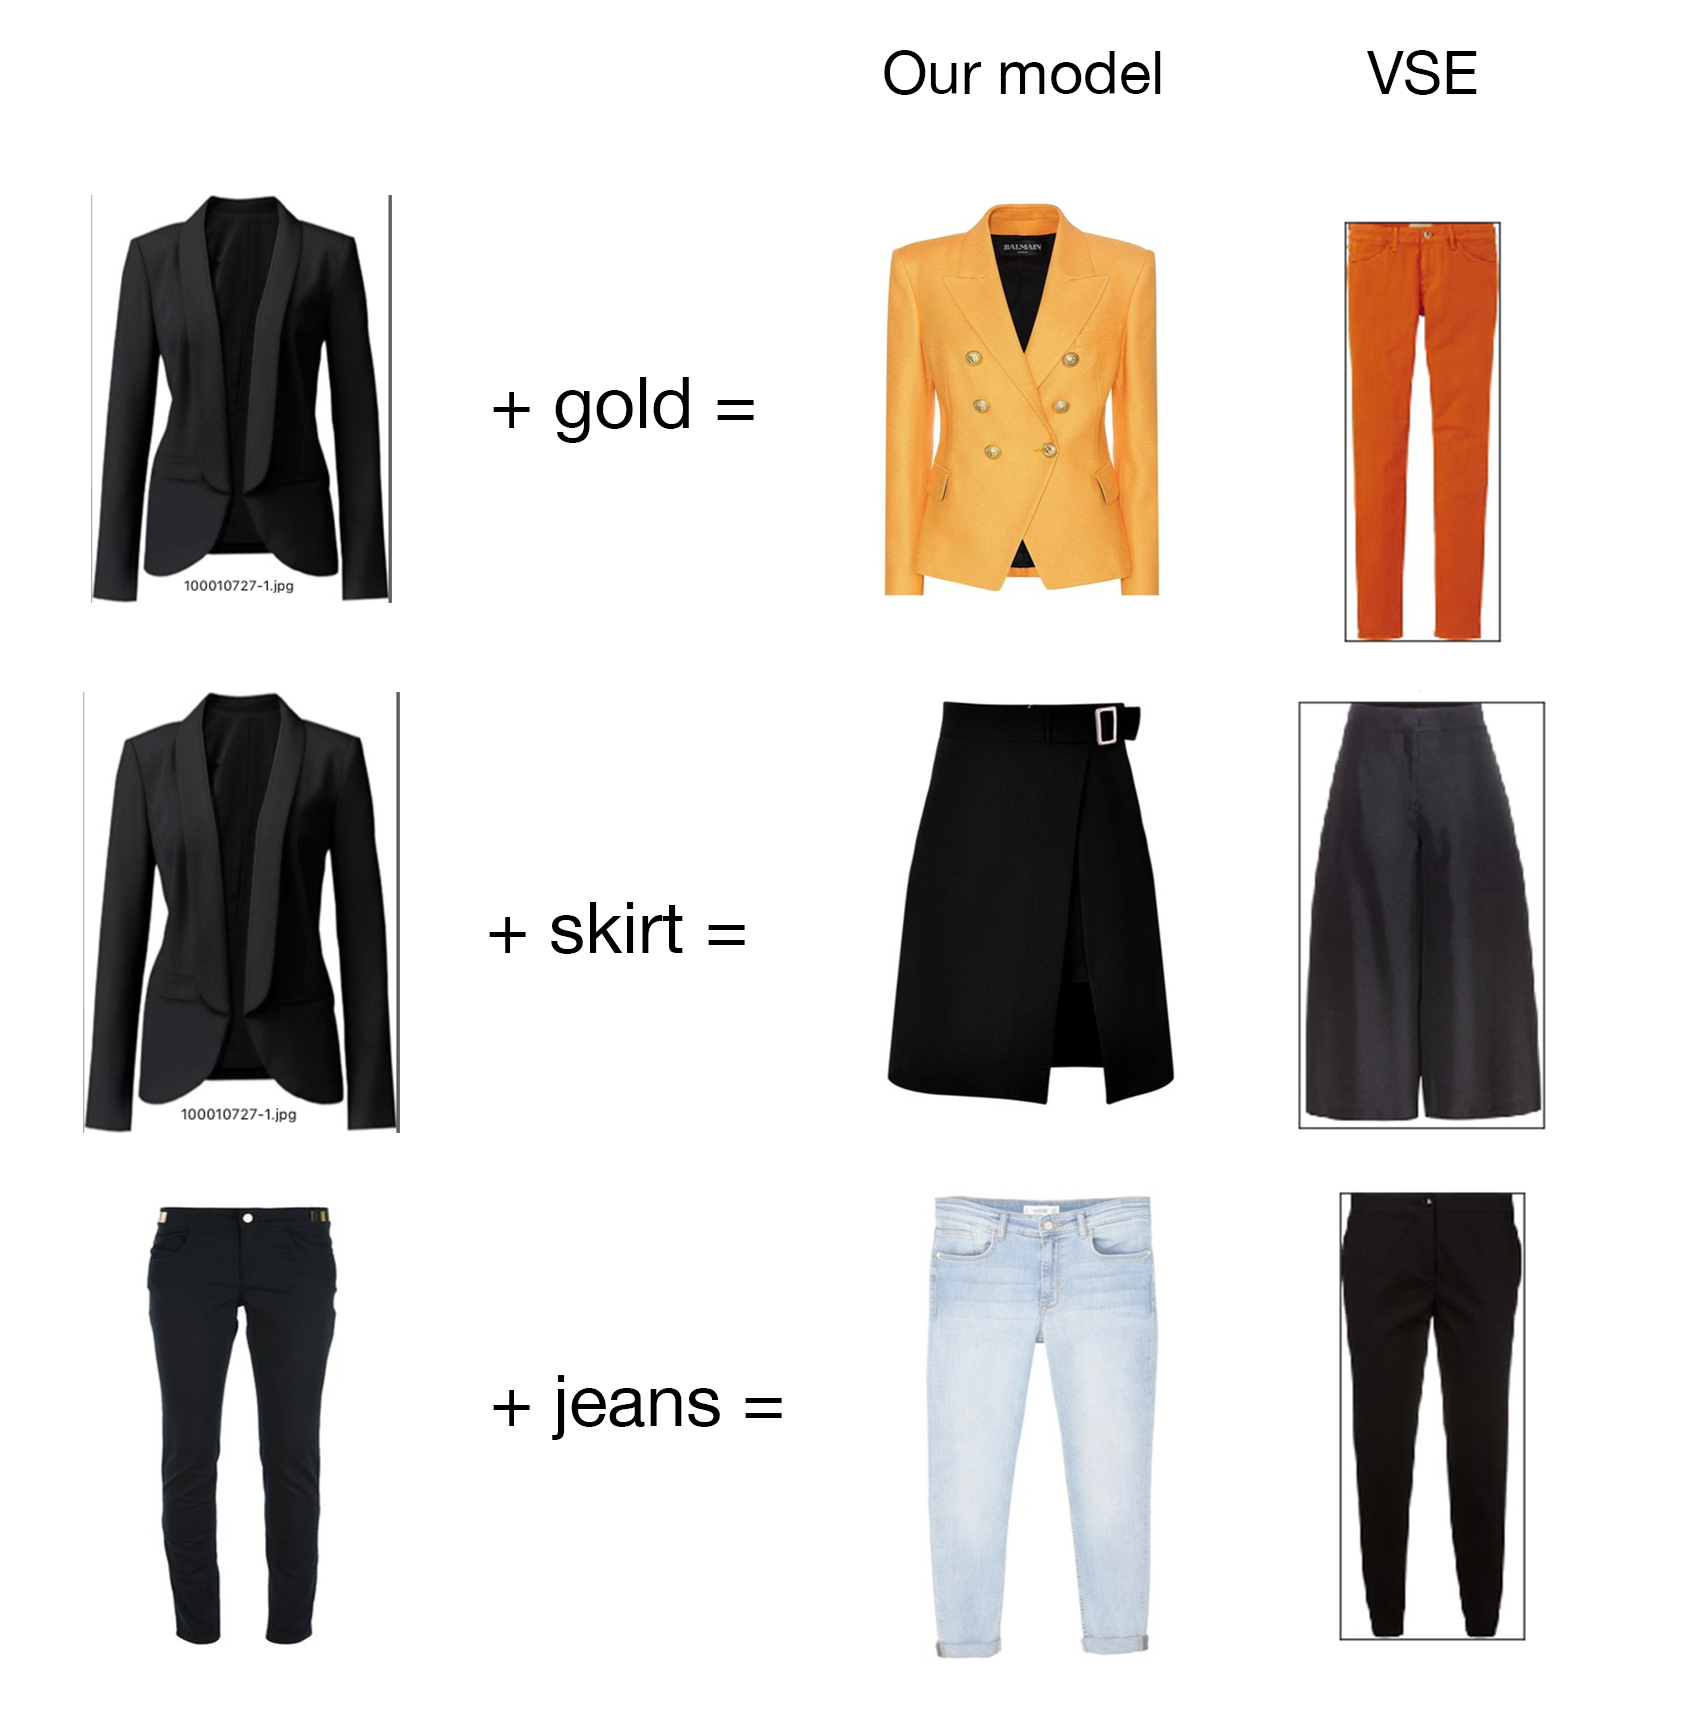
\includegraphics[width=0.56\linewidth]{images/image3.png}
    \caption{Reproduced from Tautkute et al. (2019), “DeepStyle: Multimodal Search Engine
for Fashion and Interior Design"}
    \label{fig:enter-label}
\end{figure}

The DeepStyle architecture consists of three main components:

\begin{enumerate}
    \item \textbf{Visual encoder:} A modified CNN that extracts both objective features (color, pattern, shape) and subjective style features.
    \item \textbf{Text encoder:} Processes fashion-specific descriptors and natural language queries.
    \item \textbf{Cross-modal alignment module:} Ensures that similar styles cluster together in the embedding space regardless of modality.
\end{enumerate}

The training process incorporates three types of signals:

\begin{enumerate}
    \item \textbf{Item metadata:} Includes category, brand, and designer information.
    \item \textbf{Visual attributes:} Automatically extracted from product images using computer vision techniques.
    \item \textbf{Human judgments:} Includes crowd-sourced or curated labels indicating style similarity.
\end{enumerate}

This approach allows DeepStyle to understand nuanced concepts like "bohemian," "business casual," or "avant-garde" that go beyond simple visual patterns. A user could search for "elegant evening wear with subtle patterns" and receive results that match the aesthetic intent, not just items that happen to contain the query keywords.
The model demonstrated impressive cross-modal retrieval capabilities. Users could upload an image of a garment they like and find textually similar items, or provide a text description and receive visually matching results. Furthermore, DeepStyle could perform "style transfer" searches, where a user might ask for "this dress but in a more casual style" or "shoes similar to these but more formal."
For the field of multimodal semantic retrieval, DeepStyle highlighted how domain-specific training and human-in-the-loop feedback could create retrieval systems that understand subjective dimensions. Its success in the fashion domain demonstrated the commercial potential of semantic multimodal search for e-commerce platforms where style, taste, and aesthetic appeal drive purchasing decisions.
The research also underscored the importance of building specialized embeddings that capture domain-specific semantics rather than relying solely on general-purpose visual and textual representations. This insight has influenced specialized retrieval systems in other domains where subjective attributes matter, such as interior design, art, and creative content discovery.   

\item \textbf{Probabilistic Embeddings for Cross-Modal Retrieval (2021 – Sanghyuk Chun et al.~\cite{chun2021probabilistic})} 
A profound shift has entered the representation of embeddings in multimodal retrieval systems. Rather than linking objects to fixed positions in a semantic space, these models describe objects as probability distributions-normally represented as multivariate Gaussians-in the embedding space. This probabilistic representation provides a mathematical framework to express uncertainty, something that is highly beneficial when ambiguity or partial information is present in multiple modalities.
In traditional embedding models, every image or text segment is encoded as a single vector. However, this method does not support uncertainty; hence, an imprecise image or uncertain text is still mapped to some place in the embedding space. Probabilistic embeddings overcome this by representing each item as a distribution specified by its mean vector (representing the most likely semantic location) and covariance matrix (representing the uncertainty along different dimensions).
The main developments offered by this research include:

\begin{enumerate}
\item \textbf{Uncertainty modeling:} The model can represent cases of ambiguity about an embedding. As an example, an out-of-focus image would have a "broader" distribution compared to an in-focus image, whereas an imprecise text description would have higher variance compared to an exact description.
\item \textbf{Distribution matching:} The method uses distribution divergence metrics like Kullback-Leibler divergence or Wasserstein distance as opposed to standard Euclidean or cosine distances used with point embeddings. This enables uncertainty to be managed in the retrieval process, thereby improving result ranking efficiency.

\item \textbf{Calibrated Confidence:} The confidence values produced by the model represent the level of confidence associated with the outcome of a retrieval operation. As an example, to the query of "dog on a beach," high-confidence outputs (representing a narrow distribution) will be generated where there is a strong and identifiable relationship, and low-certainty outputs where there is a wider distribution.

\item \textbf{Handling missing data:} The model effectively handles cases of missing information. When a modality is missing or weak (e.g., an image without a corresponding caption), the model assigns higher uncertainty to semantic aspects that are typically supported by that particular modality.
\end{enumerate}
In multimodal retrieval, probabilistic embeddings have several advantages. First, they allow for a more natural way of dealing with noise and uncertainty between various modalities. Second, they enable a more precise ranking mechanism by capturing different levels of confidence. Third, they provide robustness to out-of-distribution queries by properly modeling uncertainty, rather than giving overconfident predictions.
In practice, this methodology supports increased user satisfaction by distinguishing between definite and indefinite matches. An embedding-based search mechanism can report to the user, "These results unequivocally correspond to your query," as opposed to, "These can or cannot correspond; I am unsure," providing clarity about degrees of confidence.
The research also showed that probabilistic embeddings are strong in modeling the relationships between different semantic dimensions. For example, uncertainty about the presence of a "beach" in an image can be linked to uncertainty about "ocean" or "sand," thus reflecting dominant semantic relationships.
This research greatly influenced subsequent studies related to strong cross-modal retrieval and inspired approaches to address issues of unreliable and partial information in multimodal databases—a critical consideration in real-world applications where access to clean and complete information is not guaranteed.

    
\item\textbf{CLIP (2021)}  The year 2021 introduced CLIP (Contrastive Language-Image Pretraining) to the world by Radford et al. \cite{radford2021clip}. This work from OpenAI made a huge difference in the field of multimodal understanding and retrieval. Limitations of other methods, including depending on limited categorised data and their inability to understand new concepts without re-training, were eliminated.

The main feature of CLIP is the way it draws on its training methodology and size. Instead of the ImageNet-like labeled datasets, the model was trained on 400 million image-text pairs collected from the internet. Each pair consists of images and their alt-text descriptions. This allows for a wide variety of concepts compared to traditional classification datasets.

CLIP employs a dual-encoder architecture with two parallel neural networks:

\begin{enumerate}
    \item \textbf{Image encoder:} A vision transformer (ViT) or a modified ResNet that processes raw image pixels into feature representations.
    
    \item \textbf{Text encoder:} A transformer model that processes text descriptions and converts them into embeddings in the same space as the image encoder.
\end{enumerate}

Both encoders project their inputs into the same embedding space, where the training objective is contrastive: matching image-text pairs are pulled together, while non-matching pairs are pushed apart. This is implemented using a symmetric cross-entropy loss that maximizes the cosine similarity between embeddings of corresponding image-text pairs while minimizing similarity between non-matching pairs.
What makes CLIP revolutionary is its "zero-shot" transfer capability. After pretraining, CLIP can perform classification or retrieval tasks on completely new categories without any additional training. For example, if asked to classify images into "cats" and "dogs" (categories it wasn't explicitly trained on), CLIP can embed both the images and the text labels "cat" and "dog," then assign each image to the label with the highest embedding similarity.
This zero-shot capability extends to complex queries. Users can search for images using natural language descriptions like "a person standing on a mountain at sunset" or "an origami crane on a wooden table," and CLIP will retrieve relevant images even if those exact scenarios weren't part of the training data.

For semantic multimodal retrieval, CLIP represented a quantum leap in several ways:

\begin{enumerate}
    \item \textbf{Open vocabulary:} Unlike previous models constrained by fixed label sets, CLIP supports arbitrary natural language queries, making it highly flexible for real-world applications.
    
    \item \textbf{Compositional understanding:} CLIP can reason about combinations of concepts (e.g., "red car on a snowy road") thanks to its training on natural image-text pairs from the web.
    
    \item \textbf{Robustness:} Due to its diverse and large-scale web-based training data, CLIP demonstrates strong performance even under distribution shifts and noisy inputs.
    
    \item \textbf{Versatility:} CLIP supports a range of tasks such as image-to-text retrieval, text-to-image retrieval, and zero-shot classification, using the same unified model.
    
    \item \textbf{Cultural knowledge:} The model encodes general world and cultural knowledge present in the web data, allowing it to understand symbolic meanings, visual metaphors, and contextual nuances.
\end{enumerate}

The effects of CLIP are greater than academic research. It has been implemented in various applications such as image search engines, content moderation tools and AI models like DALL-E. It showed that larger-scale contrastive learning on web-scale data can help in creating powerful representations that link language and vision semantically.

Being capable of “reading” pictures and “visualizing” text made CLIP one of the most important developments in multimodal AI, paving the way for subsequent research that prioritized scale, contrastive learning, and zero-shot.

\item \textbf{ALIGN (2021)}– Jia et al. \cite{jia2021scaling} from Google Research presented ALIGN (A Large-scale ImaGe and Noisy Text model), which obtained state-of-the-art results on a variety of multimodal tasks at an unprecedented scale. Despite its similarity to CLIP, it is distinguished by its emphasis on numerous aspects, as well as its noisy web data approach.

The most important aspect of ALIGN is its training technique. Instead of filtering high-quality text-image pairs, it takes the noise of web-scale data and makes up for it with sheer quantity. The model was trained on over one billion web-sourced images and their associated alt text. This is approximately 2.5 times more data than CLIP.

ALIGN's architecture follows the dual-encoder approach:
\begin{enumerate}
    \item \textbf{Image encoder:} An EfficientNet model is used to process and extract visual features from image data, offering a balance of efficiency and accuracy.
    
    \item \textbf{Text encoder:} A BERT-based transformer encodes textual descriptions into dense semantic embeddings that align with visual representations.
\end{enumerate}

These encoders map images and text into a shared embedding space where semantic similarity can be measured. The training objective uses a contrastive loss function that maximizes similarity between paired images and texts while minimizing similarity between unpaired examples.
What makes ALIGN particularly noteworthy is its approach to data quality. Web-scraped alt-text is often noisy—it might be incomplete, contain SEO keywords, or be only tangentially related to the image content. Rather than extensively filtering this data, ALIGN's training procedure is designed to be robust to noise through:

\begin{enumerate}
    \item \textbf{Momentum contrast:} Utilizes a memory bank that stores a large queue of negative samples to enhance the effectiveness of contrastive learning.
    
    \item \textbf{Dual temperature scaling:} Applies different temperature parameters for image and text modalities to better align the respective embedding distributions.
    
    \item \textbf{Batch normalization:} Ensures training stability by normalizing the input distributions, which is especially important when dealing with noisy or uncurated web data.
\end{enumerate}

The results demonstrated that scale can indeed overcome noise. ALIGN achieved state-of-the-art performance on various zero-shot and transfer learning benchmarks, confirming that massive training on noisy data can outperform smaller but cleaner datasets.
For semantic and multimodal retrieval, ALIGN's contributions are significant:

\begin{enumerate}
    \item \textbf{Improved generalization:} Exposure to a billion-scale dataset enables the model to learn a wide array of visual and linguistic patterns, making it more capable of handling diverse inputs.
    
    \item \textbf{Robustness to real-world variation:} Training on noisy and heterogeneous web data equips the model to perform reliably in practical, unpredictable search scenarios.
    
    \item \textbf{Multilingual capabilities:} The presence of alt-text in various languages allows the model to support cross-lingual retrieval tasks, widening its usability.
    
    \item \textbf{Cultural and demographic breadth:} The breadth of data scraped from the web reflects a wide range of cultural, ethnic, and geographic contexts, increasing the model’s inclusivity and relevance.
\end{enumerate}

ALIGN taught us all an important lesson about building practical retrieval systems: It showed that embracing web-scale data, noise and all, could lead to systems that are more robust and more general than those built on carefully curated small datasets, and this lesson has influenced later work on multimodal systems, encouraging researchers to prioritize the scale and diversity of their data over its cleanliness.
ALIGN showed how “scaling beats cleaning” when it comes to multimodal learning. In doing so, it defines a way of making general-purpose semantic embeddings that can support a wide range of retrieval tasks across modalities
    

\item \textbf{CLAP (2022)} – In a study by Elizalde et al. \cite{elizalde2023clap}, the contrastive learning approach was extended to the audio domain with CLAP (Contrastive Language-Audio Pretraining). According to the study, vision-language models had made substantial progress, and the audio-language domain was often overlooked despite being a crucial aspect of comprehensive multimodal systems.
CLAP is built on the same dual-encoder backbone as CLIP, but switches out the image encoder for a dedicated audio encoder:

\begin{enumerate}
    \item \textbf{Audio encoder:} Processes audio spectrograms using either a Convolutional Neural Network (CNN) or a transformer-based architecture to generate feature embeddings.
    
    \item \textbf{Text encoder:} Functions similarly to the CLIP text encoder, transforming natural language descriptions into semantic embeddings using a transformer model.
\end{enumerate}

The model is trained on pairs of audio clips and their textual descriptions using contrastive learning. During training, the system learns to maximize similarity between matching audio-text pairs while minimizing similarity for non-matching pairs. This forces the model to understand semantic relationships between sounds and their linguistic descriptions.
Training data for CLAP includes diverse audio sources paired with captions:

\begin{enumerate}
    \item \textbf{Sound effect libraries with descriptions:} Pre-labeled sound files paired with textual annotations about the type and nature of the sounds.
    
    \item \textbf{Music with genre labels and emotional tags:} Music clips labeled with metadata such as genre (e.g., jazz, rock) and mood descriptors (e.g., happy, melancholic).
    
    \item \textbf{Audiobooks with transcripts:} Spoken word audio aligned with exact text, useful for grounding audio signals in structured language.
    
    \item \textbf{Environmental recordings with context descriptions:} Sounds from real-world environments (e.g., forests, cities) tagged with descriptive context.
    
    \item \textbf{Video soundtracks with captions or descriptions:} Audio extracted from videos, often accompanied by human-generated captions or descriptions, enriching the semantic context.
\end{enumerate}

The reason CLAP is so useful for multimodal retrieval is because of it can fill in the gap between the linguistic descriptions and the sound patterns. Users are able to find sounds using their natural language search, such as “children laughing at a playground,” “gentle rain on a metal roof,” or “upbeat jazz with saxophone,” and not have the words in the metadata.
CLAP enables several novel capabilities:

\begin{enumerate}
\item \textbf{Cross-modal audio search:} Allows users to locate audio clips that correspond to provided text descriptions, for example, “rain falling on leaves” or “children laughing.”
\item \textbf{Zero-shot audio classification:} Classify the audio sample into the desired category even when the model has never seen it during training.
\item \textbf{Audio-to-text retrieval:} An audio input is all that is needed, and this retrieves the most necessary text descriptions from a database.
\item \textbf{Semantic audio similarity:} Discovers other sounds that are similar in both acoustics and conceptually to an input, facilitating exploratory audio search and clustering.
\end{enumerate}

In comprehensive multimodal systems, CLAP acts as a vital puzzle piece. Combining with other models like CLIP, it brings users multisensory search capabilities across text, audio, and images. As a result, if a person were to search for something like a “thunderstorm,” they would be able to see images of dark clouds and lightning and listen to the sounds of raining and thunder.
The study has shown that language can be utilized as a universal bridge across sensory modalities. The text provides a common semantic space, where it is possible to align the visual concepts from CLIP and acoustic patterns from CLAP; thus, the cross-modal retrieval is performed across the three domains.
The development of CLAP allowed the invention of different contrastive learning approaches to other pairs of modalities, which suggested a general pattern for building a comprehensive multimodal understanding. Its success encouraged further research into other combinations of modality and reinforced the value of web-scale contrastive learning for semantic alignment across different forms of data.
    

\item \textbf{BLIP (2022)} – Li et al. \cite{li2022blip} introduced BLIP (Bootstrapped Language-Image Pre-training), which represents an advancement in multimodal learning as it amalgamated language-image matching with image captioning in a bidirectional relationship. CLIP is largely inclined towards matching visual and textual content as they are already paired, unlike BLIP, which can generate text to describe visuals.
The main innovation of BLIP is the bootstrapping mechanism, creating an interdependence between understanding and generation:

\begin{enumerate}
    \item \textbf{Image-caption matching:} The model initially learns to associate images with their corresponding captions, aligning their semantic representations.
    
    \item \textbf{Caption generation:} Once trained on matching, the model is used to generate new captions for images, leveraging its learned visual-language understanding.
    
    \item \textbf{Caption filtering:} Generated captions are assessed and filtered, keeping only the high-quality and semantically rich ones that best describe the images.
    
    \item \textbf{Self-training:} The filtered, high-quality captions are used as pseudo-labeled data to further train the model in a self-supervised fashion.
    
    \item \textbf{Model enhancement:} This bootstrapped cycle improves both the model’s ability to match and to generate meaningful image-text pairs.
\end{enumerate}

This bootstrapping approach addresses a critical limitation of previous systems: the scarcity of high-quality image-caption pairs. By generating its own training data, BLIP effectively expands its knowledge without requiring additional human annotation.
BLIP's architecture consists of:

\begin{enumerate}
    \item \textbf{Image encoder:} A vision transformer (ViT) encodes visual features from input images into rich embeddings.
    
    \item \textbf{Text encoder:} A transformer-based module that encodes textual descriptions, enabling semantic comparison with image embeddings.
    
    \item \textbf{Text decoder:} A transformer decoder generates natural language captions for a given image, based on the fused multimodal context.
    
    \item \textbf{Multimodal fusion layers:} These layers integrate the image and text embeddings to form a joint representation space suitable for both retrieval and caption generation tasks.
\end{enumerate}

The model is trained with multiple objectives:

\begin{enumerate}
    \item \textbf{Image-text contrastive learning:} Inspired by CLIP, this objective pulls matched image-caption pairs closer and pushes unmatched pairs apart in the embedding space.
    
    \item \textbf{Image-text matching:} A binary classification task to determine whether a given caption is the correct match for an image.
    
    \item \textbf{Language modeling:} The model is trained to generate contextually relevant and coherent captions for images using autoregressive language modeling.
    
    \item \textbf{Caption filtering:} An auxiliary module learns to evaluate the quality of generated captions and filter out those that are uninformative or incorrect.
\end{enumerate}

For semantic multimodal retrieval, BLIP offers several advantages:

\begin{enumerate}
    \item \textbf{Richer semantic representations:} By jointly optimizing contrastive, matching, and generative tasks, the model learns more nuanced and deeply connected visual-linguistic embeddings.
    
    \item \textbf{Improved zero-shot capabilities:} The generative pretraining equips the model with the ability to generalize to unseen image-text concepts without needing specific labels.
    
    \item \textbf{Explainable retrieval:} Since BLIP can generate captions for images, it provides human-understandable rationales for why an image might be relevant to a given text query.
    
    \item \textbf{Query expansion:} The captioning ability allows the model to create alternative phrasings or descriptions of queries, increasing the recall and relevance in retrieval tasks.
\end{enumerate}

BLIP also introduced an effective captioning filtering mechanism that distinguishes synthetic captions by their quality. This "capQualifier" component helps identify which generated captions are most useful for bootstrapping, preferring descriptive, accurate, and comprehensive captions over generic or inaccurate ones.
Experiments showed that BLIP outperformed previous models on image-text retrieval benchmarks while using a more efficient architecture. The bootstrapping approach proved particularly valuable for improving performance on zero-shot tasks where the model encounters new concepts not explicitly covered in its original training data.
BLIP's success demonstrated the value of combining contrastive and generative approaches in multimodal learning. By allowing the model to both understand existing associations and create new ones, BLIP represented an important step toward more comprehensive semantic understanding across modalities. This approach influenced subsequent work on multimodal foundation models that combine multiple learning paradigms to achieve more robust and versatile representations.

\item \textbf{BLIP-2: Bootstrapping Language-Image Pre-training with Frozen Image Encoders and Large Language Models} - Li et al. \cite{li2023blip2} Building on the innovations of BLIP-2 that introduced a new architecture focusing on modularity, efficiency, and leveraging pre-trained models, BLIP set a complete paradigm for both visual-semantic understanding and caption generation. In comparison, BLIP-2 is a major upgrade attained by integrating large language models (LLMs) and vision encoders through a simplified but robust intermediary.
The main innovation of BLIP-2 is its Q-Former (Query Transformer) model, which is used as an intermediate between various modalities. Instead of using one integrated model, BLIP-2 uses a more decomposed framework:

\begin{enumerate}
    \item \textbf{Frozen vision encoder}: A pre-trained vision transformer (ViT) that processes images.
    \item \textbf{Q-Former}: A transformer-based model that extracts relevant visual information through learnable queries.
    \item \textbf{Frozen language model}: A pre-trained LLM that handles text generation and understanding.
\end{enumerate}

This architecture offers several advantages:

\begin{enumerate}
    \item \textbf{Parameter efficiency}: By keeping the vision and language models frozen, training focuses only on the Q-Former.
    \item \textbf{Leverage existing specialists}: Uses the best available pre-trained models for each modality.
    \item \textbf{Flexibility}: Can swap in different vision or language models without retraining the entire system.
\end{enumerate}

The Q-Former functions as an intelligent interface that translates visual information into a format that language models can understand. It does this through a set of learnable query vectors that attend to the image features, extracting the most relevant visual information based on the task at hand.
BLIP-2 is trained in two stages:

\begin{enumerate}
    \item \textbf{Image-text contrastive learning}: The Q-Former learns to align visual and textual representations.
    \item \textbf{Visual-grounded language learning}: The Q-Former learns to generate inputs for the language model that enable it to reason about images.
\end{enumerate}

For semantic multimodal retrieval, BLIP-2 represents a significant advancement in several ways:

\begin{enumerate}
    \item \textbf{Complex reasoning}: By connecting to LLMs, BLIP-2 can perform sophisticated reasoning about visual content.
    \item \textbf{Detailed understanding}: It can answer specific questions about images rather than just retrieving based on overall similarity.
    \item \textbf{Zero-shot capabilities}: The connection to LLMs enables handling novel concepts and instructions.
    \item \textbf{Efficient indexing}: The Q-Former outputs can be indexed for fast retrieval while maintaining rich semantic representation.
\end{enumerate}

BLIP-2 shows strong performance on various tasks ranging from visual question-answering and image captioning to visual reasoning. It has the capacity, for example, to answer specific questions about images like "What safety gear is not present on this building construction site?" or "What cooking technique is shown in the photo?"
In retrieval systems, this implies progressing from shallow-matching methods to support retrieval based on deeper understanding. Users will be able to frame sophisticated questions like "Retrieve pictures showing persons who are breaking safety regulations" or "Supply examples of fusion foods that combine Mediterranean and Asian ingredients," with the design of BLIP-2 supporting the acquisition of relevant responses by reasoning instead of keyword or visual pattern recall.
BLIP-2 architecture has considerably shaped subsequent studies, and its approach has determined how specialized modules are integrated instead of building large models from the very beginning. This approach has proven highly effective, particularly with language models that grow in size and capacity, making it possible for visual systems to leverage such developments efficiently.

\item \textbf{Boon: A Neural Search Engine for Cross-Modal Information Retrieval (2023)} – In this paper, Gong et al. \cite{gong2023boon} (2023) introduced a practical search model called Boon. This paper is distinct from other multimodal models because it was specially constructed for use in shopping search scenarios where different modalities are often required to retrieve all necessary relevant information.
Boon’s major innovation is its heterogeneous information integration approach. Most e-commerce platforms keep product details in multiple formats:

\begin{enumerate}
\item \textbf{Structured metadata:} This involves categories, attributes, and technical specifications that are stored in well-defined database fields, which are important inputs for structured search and filtering.

\item \textbf{Images:} Numerous images of merchandise taken from various viewpoints, convey the appearance of a product in its totality, assisting in visual searches and user decisions.

\item \textbf{Text descriptions:} Usage of marketing copy, the list of features, and data sheets provides detailed information on each product.

\end{enumerate}

Conventional models usually consider these to be two distinct indexes; however, Boon compresses them into a uniform representation that reflects both semantic correlations and layout data.
Boon's architecture consists of several specialized encoders:

\begin{enumerate}
    \item \textbf{Image encoder:} A convolutional neural network (CNN) processes product images to extract rich visual features relevant to the product's appearance, such as shape, color, and texture.
    
    \item \textbf{Text encoder:} Transformer-based models are used to process natural language text such as product descriptions and user reviews into embeddings that capture their semantic meaning.
    
    \item \textbf{Metadata encoder:} Graph neural networks (GNNs) encode structured product attributes (e.g., size, brand, category) by modeling their interrelationships.
    
    \item \textbf{Query understanding module:} This component interprets the user’s intent across multiple modalities and reformulates it into a structured representation suitable for retrieval.
\end{enumerate}

These encoders feed into a fusion mechanism that aligns the different representations into a common semantic space while preserving their unique characteristics. This fusion is learned through multiple training objectives:

\begin{enumerate}
    \item \textbf{Relevance matching:} Determines the semantic and visual alignment between user queries and product entries to ensure accurate retrieval.
    
    \item \textbf{Category and attribute prediction:} Predicts product categories and attributes based on multimodal input to enhance search ranking and filtering.
    
    \item \textbf{Image-text alignment:} Learns to map corresponding images and descriptions to a shared embedding space, facilitating cross-modal retrieval.
    
    \item \textbf{Behavioral matching:} Leverages historical click and purchase data to model the relationship between queries and user engagement, improving personalization.
\end{enumerate}

What makes Boon particularly valuable for practical applications is its ability to handle flexible query formats. Users can search using:

\begin{enumerate}
    \item \textbf{Text-only queries:} Traditional keyword-based search where users enter natural language queries or keywords.
    
    \item \textbf{Image-only queries:} Visual search using an image as the query input, commonly employed to find similar-looking products.
    
    \item \textbf{Combined queries:} Users provide an image and refine their intent using text (e.g., “like this but in red”), enabling a more expressive search experience.
    
    \item \textbf{Faceted queries:} Combine natural language or visual input with structured filters (e.g., size, brand, color) for more precise search outcomes.
\end{enumerate}

The system also introduces an attention-based cross-modal aggregation mechanism that weighs different modalities based on query context. For instance, when a user searches for “blue dress with lace trim,” the system heavily weights color attributes for “blue” but emphasizes visual texture features for “lace trim.”
In real-world use, Boon takes advantage of smart indexing methods to bring up millions of products in a fraction of a second, even though the product representations are varied. This includes the hybrid embedding space optimized for finding nearest neighbors.
Boon shows how educational improvements on multimodal studying may be absorbed in commercial search situations where data is a combination. In particular, its achievements in product search point to the prospect of adopting it in other areas with blended data, such as real estate, job applications, or content recommendation systems.
The study explains the significance of combining behavioral indicators (clicks, acquisitions) in addition to material features, indicating that user data may serve as an implicit signal that helps align various modalities in meaningful ways.


\item \textbf{ImageBind (2023)} –Girdhar et al. \cite{girdhar2023imagebind}  from MetaAl Research introduced ImageBind, an approach that represents a significant advancement in multimodal learning by expanding beyond the traditional vision-language pairing to include multiple modalities such as images, text, audio, depth, thermal, and IMU data. ImageBind is an ambitious approach that aims to create a unified embedding space where all the modalities can be semantically aligned.


The main thought about ImageBind is that many sensory streams reveal the same information. A dog, for example, can be seen, heard, felt by heat, exists in the space, and moves in a certain way. Other systems of multimodal binding link just two concepts (like text and images), but ImageBind does both.

The innovative aspect of ImageBind is in the methodology adopted for its training. Creating datasets where all six modalities are aligned would be extremely expensive and difficult. So, the authors employed a clever trick: if modality A (images) can be aligned with modality B (text), and also with modality C (audio), then B and C can be considered as aligned with each other, since they are both aligned with modality A.
This "binding through images" approach allows ImageBind to create a unified embedding space without requiring explicit pairings between all modalities. The model is trained using only naturally occurring pairs:

\begin{enumerate}
    \item \textbf{Images paired with text captions:} Traditional image-text datasets where images are annotated with human-written or automatically generated descriptions.
    
    \item \textbf{Images paired with audio:} Sound clips recorded from the scene associated with the image, such as environmental sounds or spoken descriptions.
    
    \item \textbf{Images paired with depth maps:} Structural depth information is aligned with each image, capturing 3D spatial relationships and geometric context.
    
    \item \textbf{Images paired with thermal imagery:} Thermal data captures the temperature distribution of objects in the image, offering insight into material properties or human activity.
    
    \item \textbf{Images paired with motion data:} Dynamic movement patterns (e.g., optical flow or pose tracking) associated with the scene are recorded, providing temporal cues.
\end{enumerate}

Through contrastive learning on these paired data sources, all six modalities become aligned in a common embedding space. This means that a concept like "ocean waves" can be represented similarly whether it comes from a photograph, a text description, a wave sound recording, a depth map of water, a thermal image showing temperature gradients, or motion data capturing rhythmic movements.
For multimodal retrieval, ImageBind enables unprecedented cross-modal search capabilities:

\begin{enumerate}
    \item \textbf{Audio-to-image search:} Enables retrieval of relevant images based on sound input. For instance, the sound of waves could return photos of beaches or oceans.
    
    \item \textbf{Depth-to-text search:} Users can retrieve descriptive text based on structural and spatial features, such as identifying a room layout or object shapes from 3D depth data.
    
    \item \textbf{Motion-to-thermal search:} Allows identification of thermal imagery associated with specific motion patterns, like detecting warm footprints from walking motion data.
    
    \item \textbf{Any-to-any retrieval:} Supports flexible cross-modal search across all six modalities. For example, searching with a thermal image to find a related caption or using text to retrieve motion data.
\end{enumerate}

The experiment was conducted to determine how well ImageBind could find and retrieve various cross-modal texts between modalities, which were not seen or paired during the experiments. All the texts retrieved when the model was subjected to, for example, ‘zero-shot cross-modal retrieval between modalities’ which were never explicitly paired were considered during this test. For example, the model was capable of matching audio data and text descriptions through shared characteristics
This project has huge potential for systems that search for and retrieve meaning. It shows that systems that handle different types of information are possible - users could ask questions in different ways and be given answers in all types of forms. For example, a person might sing part of a song to find a video of a similar song, or send in a photo of a mountain to find a drawing of a mountain and a written description of it.
ImageBind also shows how different modes of communication can support one another, giving us more comprehensive ideas than just one form of communication could offer. This mirrors how real people perceive things and develop ideas.
In the realm of multimodal retrieval, ImageBind opens up future possibilities for systems that can fluidly connect numerous modalities due to their shared semantic links, thereby bringing about more natural and versatile pathways for users to discover and retrieve information across an ever-growing array of digital media.

\begin{figure}
    \centering
    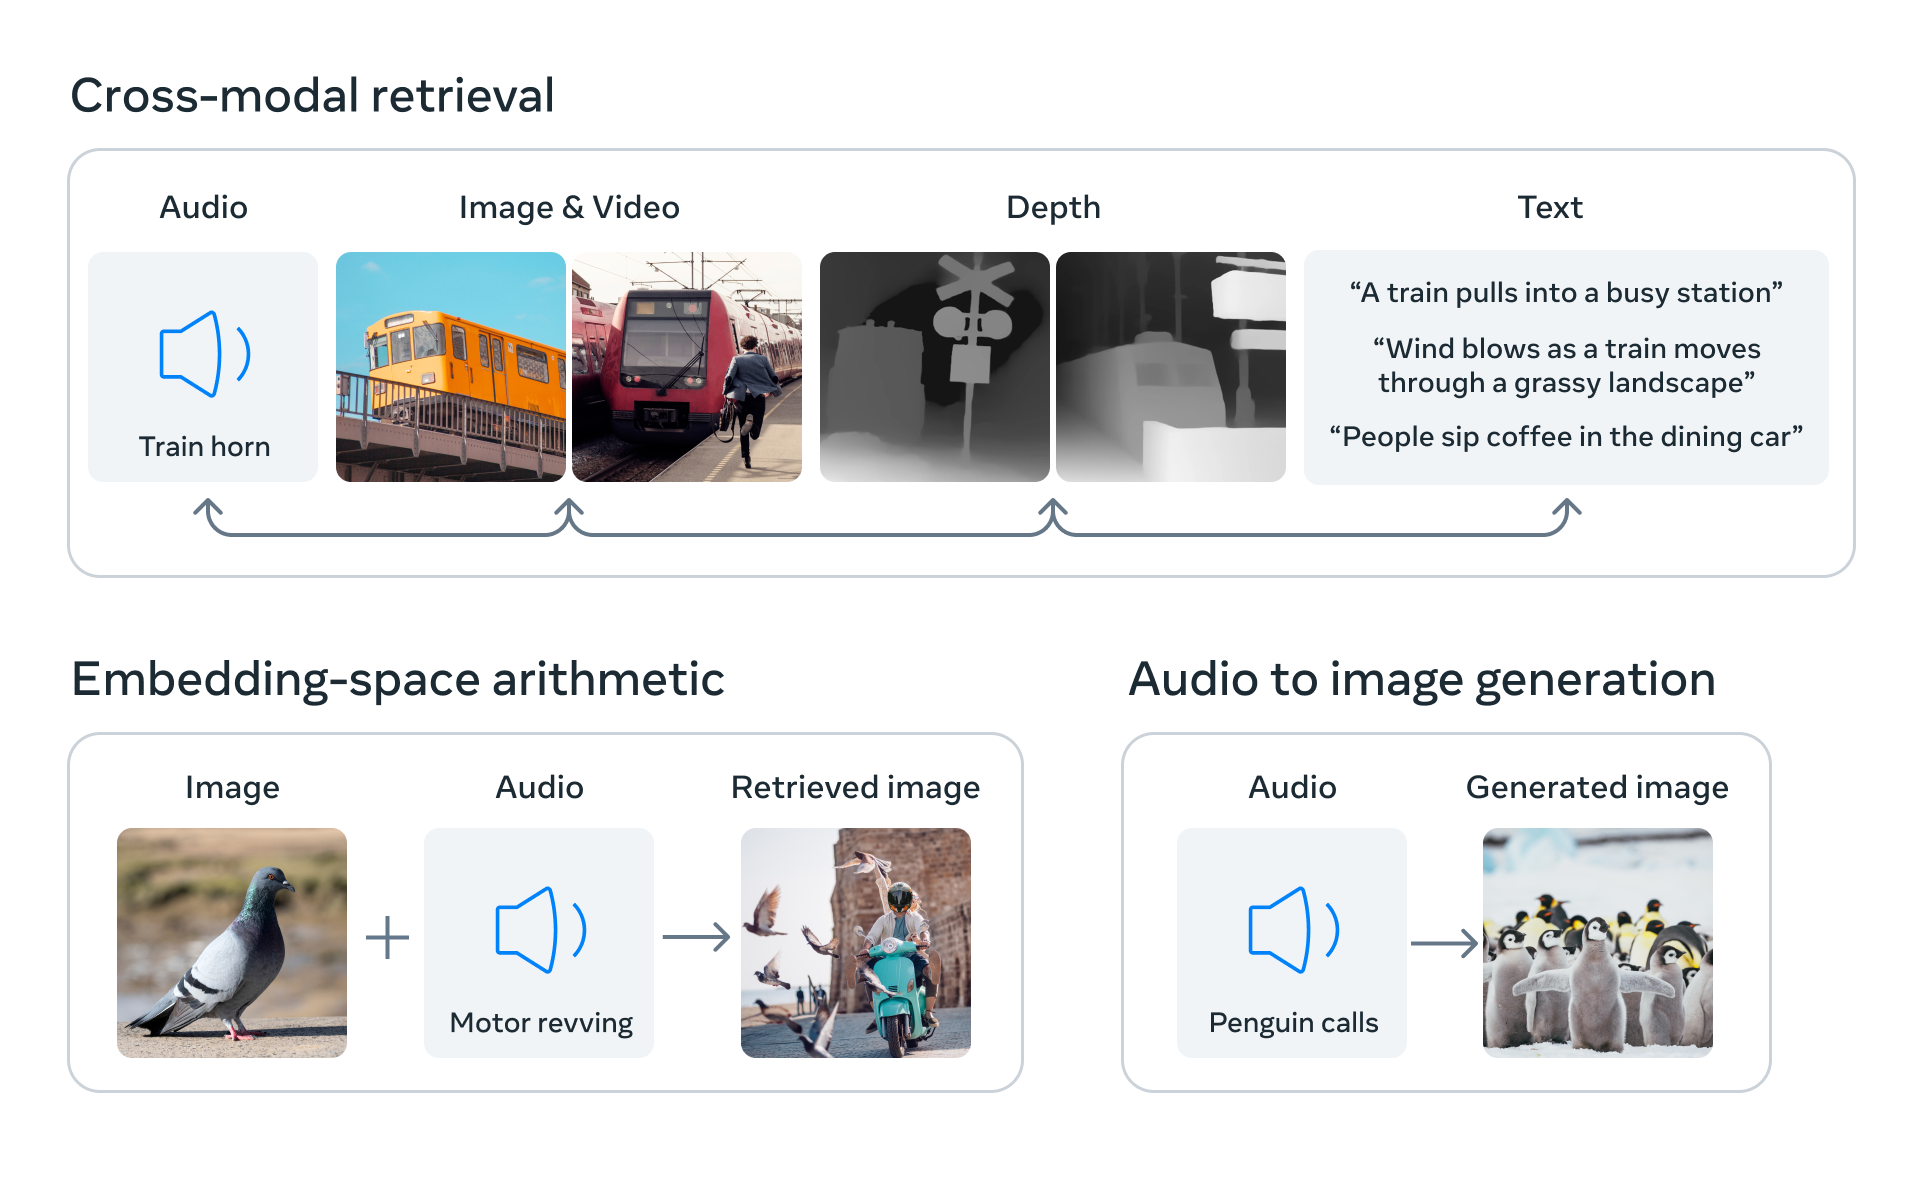
\includegraphics[width=1\linewidth]{images/image.png}
    \caption{Reproduced from Girdhar et al. (2023), “ImageBind: One Embedding Space To Bind Them All.”}
    \label{fig:enter-label}
\end{figure}

\item \textbf{Unified-IO (2023)} – Lu et al. \cite{lu2023unified} has introduced a remarkable advancement that has revolutionized the way AI tasks across different modalities are handled. It is such that it is a significant advancement over previous works that were developed specifically for certain tasks (retrieval, classification, generation, etc.) or the specific pairs of modalities. Moreover, it is general-purpose, hence treating all the tasks as sequence-to-sequence transformations.

The main concept of Unified-IO that makes all the difference is simple and straightforward. This system was developed based on the principles of several popular text-based language models. For instance, the developers used the T5 model that stands for Text-to-Text Transfer Transformer. This model works with text data only, but Unified-IO expands this concept beyond text to incorporate multimodal and image data. This approach is based on the idea that all tasks have a shared nature—they take some kind of input
Unified-IO's architecture consists of:

\begin{enumerate}
    \item \textbf{Unified encoder:} Processes input sequences that may include text, images, or a combination of both. This encoder handles multimodal fusion from the very beginning.
    
    \item \textbf{Unified decoder:} Generates output sequences that can be purely text, purely images, or multimodal sequences containing both.
    
    \item \textbf{Task specification:} A text prompt provided alongside the input to define the desired operation, such as retrieval, classification, or generation. This enables prompt-driven flexibility.
\end{enumerate}

This architecture uses a shared vocabulary and representation space across modalities, allowing the model to process text and images within the same framework. Images are treated as sequences of patches, similar to how text is processed as sequences of tokens.
What makes Unified-IO particularly powerful for retrieval is its ability to handle multiple retrieval paradigms within a single model:

\begin{enumerate}
    \item \textbf{Text-to-image retrieval:} Given a description like “Find images that show a dog playing in the snow,” the model retrieves matching visual content.
    
    \item \textbf{Image-to-text retrieval:} The model takes an image and generates descriptive text such as “A woman holding an umbrella during a rainstorm.”
    
    \item \textbf{Multimodal-to-multimodal retrieval:} Combines image and text input to find similar content, e.g., “Find scenes like this image and caption.”
    
    \item \textbf{Structured data extraction:} Given an image (e.g., a product photo), the model can extract structured fields such as product name, price, and brand.
\end{enumerate}

The model is trained on a diverse set of tasks including:

\begin{enumerate}
    \item \textbf{Image captioning}
    \item \textbf{Visual question answering}
    \item \textbf{Image classification}
    \item \textbf{Object detection and segmentation}
    \item \textbf{Visual reasoning}
    \item \textbf{Text summarization}
    \item \textbf{Text-to-image generation}
    \item \textbf{Image editing and manipulation}
\end{enumerate}

\begin{figure}
    \centering
    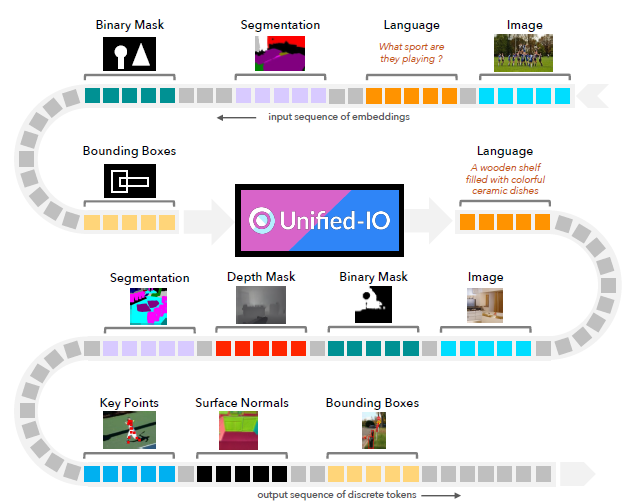
\includegraphics[width=0.75\linewidth]{images/image2.png}
    \caption{Reproduced from Lu et al. (2023), “Unified IO: A UNIFIED MODEL FOR VISION, LANGUAGE, AND MULTI-MODAL TASKS”}
    \label{fig:enter-label}
\end{figure}

Unified-IO acquires a deep understanding of semantic relationships across domains by mastering all of these tasks at the same time. This multi-task learning approach requires the model to develop general-purpose representations that embody the true meaning of information, rather than being restricted to specific use-cases.
For semantic retrieval specifically, Unified-IO offers several advantages:

\begin{enumerate}
    \item \textbf{Flexibility:} A single model supports many types of retrieval and generation tasks across different modalities.
    
    \item \textbf{Reasoning-enhanced retrieval:} The model is capable of inserting reasoning steps between query interpretation and retrieval, improving semantic alignment.
    
    \item \textbf{Explanations:} It can generate natural language explanations that justify why a particular item was retrieved or generated.
    
    \item \textbf{Zero-shot adaptation:} The model generalizes to new retrieval tasks without needing task-specific retraining, thanks to prompt-driven conditioning.
\end{enumerate}

The architecture also allows for compositional queries that combine retrieval with other operations. For example, a user might request "Find images of beaches, then describe the weather conditions in each," and Unified-IO would handle both the retrieval and analysis steps.
Experiments showed that Unified-IO achieved strong performance across 20 diverse vision and language tasks despite using a single model rather than specialized architectures for each task. This demonstrated the power of the unified sequence-to-sequence approach for multimodal understanding.
For the field of multimodal retrieval, Unified-IO points toward more integrated systems where retrieval is not isolated from other operations but part of a continuous spectrum of ways to transform and interact with information. Its task-agnostic philosophy suggests that future retrieval systems might adapt more fluidly to user needs, handling traditional search alongside generation, editing, analysis, and reasoning as part of a seamless interaction paradigm.

\item \textbf{Universal Vision-Language Dense Retrieval (2023)} – Liu et al. \cite{liu2023univldr}, which introduced a framework for Universal Vision-Language Dense Retrieval, which aimed to solve a critical problem in multimodal search: how to construct a general-purpose retrieval model that could work well on diverse benchmarks and datasets without extensive fine-tuning on many tasks.

The main innovation in this work is a training technique that combines three major elements:
\begin{enumerate}
    \item \textbf{Hard negative mining:} Using challenging negative examples that are semantically related but do not match.
    \item \textbf{Domain adaptation techniques:} Methods to generalize across different data distributions.
    \item \textbf{Contrastive representation learning:} Learning discriminative embeddings that maintain semantic relationships.
\end{enumerate}

The architecture follows the \textbf{dual-encoder paradigm} common in dense retrieval:

\begin{enumerate}
    \item A \textbf{vision encoder} processes images into fixed-length vectors.
    \item A \textbf{text encoder} processes queries into vectors of the same dimensionality.
    \item \textbf{Similarity} between these vectors determines retrieval ranking.
\end{enumerate}

What distinguishes this approach is its training procedure, which incorporates:

\textbf{In-batch negatives with temperature scaling:} Instead of using only explicitly defined negative examples, this method treats all other examples in a training batch as negatives. The distinction between positives and negatives is controlled by the temperature parameter, which must be used carefully to avoid underfitting or overfitting.

\textbf{Cross-dataset mixing}: When training, this system processes groups of examples that are taken from different sets of data, where each set can pertain to a different domain, such as various categories of images or other forms of data. As multiple types of information are presented to the system, it can learn certain features that do not change between the

\textbf{Momentum contrast with large queues}: The technique functions with the assistance of a memory bank that is used to store past encoded samples to provide a more extensive contrast pool size without a need to alter the batch size. This primarily helps the model to determine the difference, no matter how small, between semantically related features.

\textbf{Adaptive margin loss}: The similarity threshold is determined dynamically by the complexity of the examples, which makes it possible to strictly distinguish between simple cases and relax this requirement for difficult cases.

For multimodal retrieval, this universal approach offers several practical advantages:

\begin{enumerate}
    \item \textbf{Deployment efficiency:} A single model handles multiple retrieval scenarios without the need for separate specialized models.
    
    \item \textbf{Zero-shot capabilities:} The model performs reasonably well on new datasets without additional fine-tuning.
    
    \item \textbf{Resource optimization:} Computes and stores a single embedding per item for efficient indexing and retrieval.
    
    \item \textbf{Consistency:} Employs the same similarity measure across diverse content types and query formats.
\end{enumerate}

Tests unveiled that this common search engine has the competence to outdo or equal specialized models on several yardsticks, even on MSCOCO, Flickr30K, and Visual Genome. A point of note is the machine’s brilliance in switching to unseen databases and still retaining the same high quality.
The research work similarly launched a thoroughgoing analysis of what makes retrieval “universal”, unveiling essential factors, just like embedding dimensionality, training data variety, and optimizing strategies that cause cross-domain generalization.
This work is a significant milestone in the development of practical and functional multimodal retrieval systems. Instead of having to design a new system every time you come across a new domain, a universal retrieval system might be enough. The versatility of this universal model is particularly beneficial in real-world applications due to the constant need to perform additional operations.

\item \textbf{Multimodal Semantic Retrieval for Product Search (2025)} – Liu et al. \cite{liu2025multimodal} developed a specialized multimodal retrieval system that focuses on the unique challenges of e-commerce product search. While sharing some goals with Boon, this work places particular emphasis on user behavior signals and personalization aspects of product retrieval.
The core insight of this research is that product search differs fundamentally from general information retrieval in several ways:

\begin{enumerate}
    \item \textbf{Intent diversity:} Users may interact with the system for different reasons—browsing casually, comparing options, or intending to purchase—which affects how relevance should be interpreted.
    
    \item \textbf{Preference subjectivity:} What is relevant or attractive to one user may not be the same for another, as personal taste, brand loyalty, and style preferences vary greatly.
    
    \item \textbf{Multimodal decision factors:} Users make decisions based on a combination of visual appearance, textual specs, pricing, and social proof (like reviews), necessitating holistic modeling.
    
    \item \textbf{Session context:} The user's previous actions within a session—like recently viewed or clicked products—can dramatically influence what is deemed relevant in subsequent queries.
\end{enumerate}

To address these challenges, the researchers designed a dual-encoder architecture with several innovations:

\begin{enumerate}
    \item \textbf{Behavioral embedding layer:} This module captures user-specific preferences by encoding historical interactions, such as previous clicks, purchases, and browsing behavior.
    
    \item \textbf{Visual attention module:} Identifies and focuses on the most relevant parts of product images (e.g., logos, color patterns) based on the user's current query and interest signals.
    
    \item \textbf{Preference modeling:} Learns a user profile from historical behavior, helping tailor search results toward an individual’s unique taste, brand affinity, and stylistic preferences.
    
    \item \textbf{Multi-task learning:} Trains the model simultaneously on multiple tasks—such as click-through rate prediction, purchase likelihood, and general relevance—to encourage robust and comprehensive personalization.
\end{enumerate}

The training methodology combines multiple signals:

\begin{enumerate}
    \item \textbf{Click data:} Indicates the user's initial interest and serves as a weak signal for relevance.
    
    \item \textbf{Purchase data:} Represents strong implicit feedback, indicating that the product met user expectations in multiple dimensions.
    
    \item \textbf{Browse time:} Longer engagement time often correlates with greater user interest or consideration.
    
    \item \textbf{Add-to-cart actions:} Suggests serious purchase intent and serves as a midpoint between interest and conversion.
    
    \item \textbf{Product-to-product co-views:} If users commonly view certain products together, it implies perceived similarity and can inform recommendations and related-product retrieval.
\end{enumerate}

What distinguishes this work is its holistic approach to relevance. Rather than treating relevance as a fixed property of query-item pairs, it models relevance as a function of:

\begin{enumerate}
    \item \textbf{Query content:} The semantics of the user’s query provide a starting point for determining relevance, especially in natural language input.
    
    \item \textbf{Product features (visual and textual):} Visual cues (like color, shape) and textual information (like brand, description) are matched against the user’s preferences.
    
    \item \textbf{User preferences:} Derived from long-term behavior and profile data, preferences help personalize results for recurring users.
    
    \item \textbf{Session context:} Incorporates immediate actions (clicks, views) to adapt relevance dynamically during the same search session.
    
    \item \textbf{Stage in the purchase journey:} Early-stage users may be exploring broadly, while late-stage users (who’ve added to cart or spent time comparing) need more targeted and decision-supportive results.
\end{enumerate}


In the broad realm of multimodal retrieval studies, this study showcases the role played by behavioral cues in bridging the gap between different modalities. Whenever a user clicks upon a product after a particular query, it suggests that there is a semantic connection between the query terms and the product image, which can help the model learn about cross-modal associations.
The system brings in a self-adjusting fusion mechanism that gages various modalities based on technology and user history. For instance, for searches such as "red dress," the fusion would lean more on the visual element as against searches like "waterproof camera," where other specification elements are scrutinized to a greater extent.
Research has revealed that including the behavior of users has a significant impact on cross-model retrieval optimization compared to the use of content-based algorithms. The result was better, not only maximizing the user’s perceived beliefs.
This work underlines the importance of expanding the focus of multimedia retrieval systems from content understanding to the incorporation of user intent and preferences, particularly in cases where subjective factors play a role in determining relevance. Its results are relevant for personalizing content recommendations and discovery in various sectors, including content recommendations, personalized learning resources.

\end{enumerate}

\section{Discussion}

The path of study in semantic and multimodal information retrieval shows a rich tapestry of changing ideas, techniques, and uses. Spanning more than a decade, from basic studies like \textbf{DeViSE} to modern large-scale systems like \textbf{BLIP-2} and \textbf{ImageBind}, the 18 research papers previously covered. This part looks at the links between these works critically, noting common themes, contrasting approaches, and investigating how they complement, diverge from, or build upon one another. The aim is to highlight not only personal contributions but also how these combine to influence the larger scene of semantic and multimodal retrieval.

\subsection{The Rise of Contrastive Learning in Multimodal Retrieval: From CLIP to BLIP-2}

By allowing strong alignment between various modalities—especially text and vision—without demanding fine-grained supervision, the arrival of contrastive learning fundamentally changed multimodal information retrieval. A lineage of models including \textbf{CLIP (2021)}, \textbf{ALIGN (2021)}, \textbf{BLIP (2022)}, and \textbf{BLIP-2 (2023)} best illustrates this change. Although they all have a common motif of projecting text and image data into a shared embedding space, their designs, training techniques, and intended applications expose significant variations.

CLIP pioneered the dual-encoder contrastive paradigm at web scale. It trained a text encoder and an image encoder independently using a sizable corpus of noisy image-text pairs that were collected from the internet, aligning their outputs using a contrastive loss. This method was scalable and elegant, allowing open-vocabulary image search and zero-shot image categorization without the need for task-specific fine-tuning. The model's adaptability led to a surge in related studies.

The same dual-encoder methodology was used by Google Research's ALIGN, which was unveiled that same year but trained on more than a billion image-text pairs. ALIGN accepted the noise and depended on the large volume of data and strong training objectives to generalize, whereas CLIP used some filtering of its web data to ensure quality. This method supported the idea that noise can be reduced by scale, a lesson that informed later multimodal models.

BLIP marked a small but crucial development. Instead than depending exclusively on contrastive objectives, it added caption creation and self-training into its learning process. Because of this, BLIP was a hybrid system that could produce and comprehend natural language. It was able to bootstrap high-quality image-caption pairs through its self-training loop, which enhanced semantic grounding and made tasks like captioning and visual question responding possible in addition to retrieval. This comprehensive method expanded the use of multimodal models beyond retrieval to include generation and reasoning.

BLIP-2 extended this concept with an architectural innovation—the Q-Former, a learnable intermediary module that connects a frozen vision encoder to a frozen large language model (LLM). This modular design reflects a major trend in contemporary AI: leveraging the strengths of independently trained foundation models through lightweight bridges. BLIP-2’s ability to perform visual reasoning, answer open-ended questions about images, and generate coherent natural language outputs without training a monolithic end-to-end model highlights the power of modularity and pretraining synergy. It also marks a shift from \textit{alignment} (CLIP, ALIGN) to \textit{interpretation and reasoning} (BLIP-2).

In comparing these models, several key distinctions emerge:

\begin{enumerate}
  \item \textbf{Training paradigm}: CLIP and ALIGN focus on alignment through contrastive loss; BLIP incorporates generative objectives; BLIP-2 introduces modular fusion with LLMs.
  
  \item \textbf{Architecture}: Dual encoder (CLIP, ALIGN), unified encoder-decoder (BLIP), modular vision-language bridge (BLIP-2).
  
  \item \textbf{Capabilities}: CLIP and ALIGN excel at open-vocabulary retrieval; BLIP and BLIP-2 add generation, reasoning, and VQA.
  
  \item \textbf{Scalability}: ALIGN emphasizes scale and robustness to noise; BLIP and BLIP-2 emphasize data efficiency through self-training and modularity.
\end{enumerate}

Together, these models trace the arc of multimodal AI from alignment to understanding to reasoning, each pushing the envelope of what retrieval systems can achieve.

\begin{table}[ht]
\centering
\caption{Large-Scale Contrastive Models Comparison}
\label{tab:contrastive}
\small
\setlength{\tabcolsep}{4pt}
\begin{tabularx}{\columnwidth}{@{}>{\raggedright\arraybackslash}X>{\raggedright\arraybackslash}X>{\raggedright\arraybackslash}X>{\raggedright\arraybackslash}X>{\raggedright\arraybackslash}X@{}}
\toprule
\textbf{Feature} & \textbf{CLIP (2021)} & \textbf{ALIGN (2021)} & \textbf{BLIP (2022)} & \textbf{BLIP-2 (2023)} \\
\midrule
Architecture & Dual encoder (ViT + Text) & Dual encoder (EfficientNet + BERT) & Encoder-decoder & Modular (ViT + Q-Former + LLM) \\
Training Data & 400M web pairs & 1B web pairs & Filtered + generated & Bootstrapped + frozen LLM \\
Objectives & Contrastive & Contrastive & Contrastive + generation & Contrastive + reasoning + generation \\
Zero-shot & Yes & Yes & Yes & Yes \\
Generation & No & No & Yes & Yes \\
Reasoning & No & No & Basic & Yes \\
Strengths & Simplicity & Scale & Generative & Modular reasoning \\
\bottomrule
\end{tabularx}
\end{table}

\subsection{Beyond Point Embeddings: Polysemy, Uncertainty, and Contextual Nuance}

Meaning is at the heart of semantic retrieval. However, meaning is rarely solitary or fixed, particularly in perception and natural language. By going beyond the presumption that an input corresponds to a single point in the embedding space, two works—\textbf{Polysemous Visual-Semantic Embeddings (2019)} and \textbf{Probabilistic Embeddings for Cross-Modal Retrieval (2021)}—address this difficulty directly.

The problem of \textit{polysemy}, in which a single word can have several meanings depending on context, is addressed in \textbf{Song et al. (Polysemous VSE)}. They suggest a technique in which words are stored into several sense-specific embeddings rather than into a single vector. Which sense is relevant depends on the situation, whether it be visual or written. This method makes fine-grained disambiguation possible. An image of a riverbank, for instance, will be more in line with the "riverside" meaning of "bank," not the financial

\textbf{In contrast, Chun et al. use a probabilistic approach, describing every item in the embedding space as a multivariate Gaussian. A crisp, well-annotated sample has a sharper, more confident distribution, whereas a hazy or ambiguous image is represented with a broader distribution thanks to this innovation, which allows the model to communicate uncertainty. Thus, retrieval is no longer just about comparing vectors but also about comparing distributions.}

Although they do so from distinct perspectives—one by discrete multiplicity, the other by continuous uncertainty—both strategies seek to represent contextual ambiguity and confidence. Crucially, both improve semantic richness, laying the groundwork for systems that are not just accurate but also truthful about their accuracy—a crucial component for reliable retrieval in high-stakes fields like law or medicine.


\begin{table}[ht]
\centering
\caption{Disambiguation and Uncertainty Models}
\label{tab:uncertainty}
\small
\setlength{\tabcolsep}{4pt}
\begin{tabularx}{\columnwidth}{@{}>{\raggedright\arraybackslash}X>{\raggedright\arraybackslash}X>{\raggedright\arraybackslash}X@{}}
\toprule
\textbf{Feature} & \textbf{Polysemous VSE (2019)} & \textbf{Probabilistic Embeddings (2021)} \\
\midrule
Focus & Word sense disambiguation & Uncertainty modeling \\
Method & Multi-sense embeddings & Gaussian distributions \\
Disambiguation & Visual/text context & Variance-based \\
Strength & Fine-grained matching & Confidence-aware \\
Use Case & Polysemous queries & Noisy/missing data \\
\bottomrule
\end{tabularx}
\end{table}

\subsection{Cross-Modal Transformers and Unified Representations}

The emergence of \textbf{transformer architectures} catalyzed the development of joint multimodal processing systems, moving beyond late fusion of modality-specific features to deep, shared understanding. Early in this trend was \textbf{VisualBERT (2019)}, which fused image region features and word tokens into a shared transformer sequence. This allowed for cross-modal self-attention, enabling the model to learn rich relationships such as “this object is the subject of that caption.”

\textbf{Unified-IO (2023)} took this one step further by proposing a \textbf{task-agnostic, sequence-to-sequence framework} that handles a wide variety of inputs (text, images) and outputs (text, classification labels, bounding boxes). All tasks are cast as sequence transformations, inspired by T5’s “text-to-text” format. The model doesn’t just retrieve or classify—it can \textbf{describe, reason, detect, and explain}. Unified-IO embodies a vision of multimodal generality, where retrieval is not a distinct task but one capability among many in a unified generative system.

\textbf{ImageBind (2023)}, from Meta, offers a more radical unification—not of tasks, but of \textbf{modalities}. It simultaneously embeds six modalities (image, text, audio, depth, thermal, motion) into a single space. The innovation lies in its training strategy: it does not require all modalities to be seen together. Instead, it uses images as a semantic pivot, binding other modalities indirectly. This means that sound can be linked to text via shared image contexts, even if the model never saw sound-text pairs directly.

Together, these three models—\textbf{VisualBERT}, \textbf{Unified-IO}, \textbf{ImageBind}—form a compelling triad:

\begin{enumerate}
  \item \textbf{VisualBERT}: Early cross-modal attention; focuses on text and vision.
  \item \textbf{Unified-IO}: Task-unified, transformer-based reasoning; general-purpose.
  \item \textbf{ImageBind}: Modality-unified, contrastive learning; scalable to sensory data.
\end{enumerate}

They collectively mark the transition from retrieving information to reasoning across modalities, and ultimately to perceiving and acting across sensory experiences.

\begin{table}[ht]
\centering
\caption{Unified and Transformer-Based Models}
\label{tab:transformers}
\small
\setlength{\tabcolsep}{4pt}
\begin{tabularx}{\columnwidth}{@{}>{\raggedright\arraybackslash}X>{\raggedright\arraybackslash}X>{\raggedright\arraybackslash}X>{\raggedright\arraybackslash}X@{}}
\toprule
\textbf{Feature} & \textbf{VisualBERT (2019)} & \textbf{Unified-IO (2023)} & \textbf{ImageBind (2023)} \\
\midrule
Input Modalities & Image+Text & Image+Text & 6 modalities \\
Architecture & Joint transformer & Seq-to-seq & Contrastive \\
Task Scope & Retrieval, VQA & Generation & Any-to-any \\
Objective & Masked modeling & Multi-task & Contrastive \\
Strengths & Cross-attention & Flexibility & Modality scaling \\
\bottomrule
\end{tabularx}
\end{table}

\subsection{Domain Specialization and Real-World Applications}

General-purpose models are powerful, but domain-specific applications demand tailored solutions. \textbf{DeepStyle} models subjective fashion styles using crowd data. \textbf{Boon} integrates structured metadata and behavior for e-commerce retrieval. The \textbf{2025 multimodal product search system} introduces adaptive fusion and personalized ranking.

\begin{table}[ht]
\centering
\caption{Domain-Specific Systems}
\label{tab:domain}
\small
\setlength{\tabcolsep}{4pt}
\begin{tabularx}{\columnwidth}{@{}>{\raggedright\arraybackslash}X>{\raggedright\arraybackslash}X>{\raggedright\arraybackslash}X>{\raggedright\arraybackslash}X@{}}
\toprule
\textbf{Feature} & \textbf{DeepStyle (2019)} & \textbf{Boon (2023)} & \textbf{Product Search (2025)} \\
\midrule
Domain & Fashion & E-commerce & E-commerce \\
Modalities & Img+Txt & Img+Txt+Meta & Img+Txt+Behavior \\
Personalization & Aesthetic clusters & Click data & Session+profile \\
Task & Style search & Ranking & Personalized \\
Strengths & Subjective matching & Metadata fusion & Adaptive \\
\bottomrule
\end{tabularx}
\end{table}

\subsection{From Semantic Search to Multimodal Reasoning}

A final thread that runs through this body of work begins not with images, but with semantics in text. The work of \textbf{Bast et al. (2016)} on semantic search in knowledge bases introduced ideas that are surprisingly relevant to modern multimodal models: entity linking, semantic parsing, hybrid reasoning. Their system mapped natural language queries into structured logical forms, enabling precise, entity-aware search.

This textual infrastructure laid the groundwork for modern \textbf{vision-language models} that must do similar reasoning—but across modalities. \textbf{BLIP-2} connects visual inputs to LLMs, effectively treating images as structured prompts. \textbf{Unified-IO} translates multimodal inputs into structured outputs. Even models like \textbf{ImageBind} benefit from the knowledge-structuring traditions in NLP, as they rely on text as a bridge modality.

Thus, a surprising lineage emerges: from symbolic, entity-centric text search, to neural, perception-aware multimodal reasoning. It reflects an enduring tension—and a growing synthesis—between structured knowledge and unstructured perception, between logic and learning.

\section{Conclusion}

The evolution of semantic and multimodal information retrieval has been marked by three parallel expansions: of scale, of modality, and of capability. Models have grown from small, task-specific systems to massive, general-purpose engines capable of zero-shot reasoning across text, image, and sound. Architectures have shifted from late fusion pipelines to joint transformer backbones and modular pretraining strategies. Most importantly, the definition of retrieval itself has changed—from finding similar items to understanding, interpreting, and explaining across modalities.

Yet challenges remain. Questions of \textbf{interpretability}, \textbf{bias}, \textbf{energy consumption}, and \textbf{fairness} loom large. Moreover, as systems like \textbf{ImageBind} promise “\textit{any-to-any}” retrieval, new questions emerge: \textit{How do we evaluate such models? How do we design interfaces that allow users to express complex cross-modal intents?}

Nevertheless, the field has moved decisively toward a future where semantic understanding is not modality-specific, but unified, robust, and grounded in rich embeddings shaped by both data and human context. The works surveyed here do not merely contribute individual innovations—they form a collective foundation for the next generation of information retrieval systems: systems that can see, hear, read, reason—and ultimately, understand.


\bibliographystyle{IEEEtran}
\bibliography{references}

\end{document}